
\documentclass[12pt,a4paper]{report}
\usepackage{graphicx}
\usepackage{amsmath}
\usepackage{amssymb}
\usepackage{listings}
\usepackage{url}
\usepackage{dirtree}
\usepackage[usenames]{color}


\begin{document}

%%=================================================================================
%%Front page

\thispagestyle{empty}

\begin{titlepage}

\vspace*{1.0cm} 
    \begin{center}
      \line(1,0){350}\\
      \LARGE
      \textbf{NiftyRec @Nifty_Rec_VERSION_MAJOR@.@Nifty_Rec_VERSION_MINOR@}\\
      \large
      \textbf{Software Guide}\\
      \vspace{1.0cm}
      \small \today \\
      \line(1,0){350}\\
    \end{center}

    \begin{figure}[!h]
      \begin{center}
        
\includegraphics[width=3.0cm]{niftyrec_logo}
      \end{center}
    \end{figure}


\vspace*{4.0cm} 
\large
\begin{flushright}
  Alexandre Bousse\\
%  Manuel Jorge Cardoso\\
  Marc Modat\\
%  Matt Clarkson\\
%  Pankaj Daga\\
  Sebastien Ourselin\\
  Stefano Pedemonte\\
\end{flushright}

\vspace*{1.5cm}
  \begin{figure}[htbp]
    \begin{flushright}
      
\includegraphics[width=4.3cm]{logo_cmic}
    \end{flushright}
  \end{figure}

\end{titlepage}

%%=================================================================================
%%Table of contents

\tableofcontents

%%=================================================================================
%%Introduction

\chapter{Introduction}

\section{Overview}

NiftyRec provides routines for Emission Tomographic reconstruction. 
The software is written in C and computationally intensive functions have a 
GPU accelerated version based on NVidia CUDA.
NiftyRec includes a mex-based Matlab Toolbox and a Python module that 
provide easy to the low level routines for reconstruction, hiding the complexity of C and 
of the GPU accelerated algorithms, while maintaining the full speed. 
Fast projection and backprojection with depth-dependent collimator and detector response and 
attenuation correction are at the core of NiftyRec. 
NiftyRec has been designed for performance, ease of use, modularity, accessibility of the code and portability.


\section{Feature List}

\noindent {\bf Projector and Backprojector}
\begin{itemize}
  \item Depth-dependent Point Spread Function (DDPSF)
  \item Attenuation correction
  \item Rotation based ray-tracing
  \item FFT based convolution
  \item GPU acceleration
\end{itemize}

\noindent {\bf Reconstruction algorithms}
\begin{itemize}
  \item Maximum Likelihood Expectation Maximization (MLEM)
  \item Ordered Subsets Exectation Maximization (OSEM)
  \item One-step-late Maximum a-posteriori Expectation Maximization (OSL-MAPEM)
  \item Gradient ascent Maximum Likelihood and Maximum a-posteriori
\end{itemize}

\noindent {\bf Priors}
\begin{itemize}
  \item Total variation
  \item Joint Entropy based anatomical prior
\end{itemize}

\noindent {\bf Scatter Correction}
\begin{itemize}
  \item Reconstruction Based Scatter Correction (RBSC)
\end{itemize}

\noindent {\bf Bindings}
\begin{itemize}
  \item Matlab
  \item Python
\end{itemize}

\noindent {\bf Miscellaneous functions}
\begin{itemize}
  \item Generate 3D synthetic phantoms
  \item Load and write DICOM and NIFTY files
  \item GPU accelerated 3D affine transformation
\end{itemize}


\section{Algorithms}
\subsection{Projection and Backprojection}
Iterative reconstruction methods based on a stochastic model of the emission process \cite{shepp_1982,qi_2006,borman_2004} 
have been widely shown to provide better image quality than analytic reconstruction \cite{johnson_1997,frese_2003}. 
The reason for the improvement in image quality is that photon count statistics are taken in account in the model of the 
imaging system; furthermore stochastic methods facilitate the inclusion of complex system models that take into account 
detailed collimator and detector response (CDR). 

\noindent The CDR, including collimator geometry, septal penetration and detector response, may be taken
into account in a stochastic reconstruction algorithm in the form of a Point
Spread Function (PSF) that modulates the response of an
ideal Gamma Camera \cite{zeng_1992}\cite{rahmim_2008}.

\noindent The computational complexity associated with stochastic reconstruction methods however still limits their application 
for clinical use and inclusion of complex system models further increases the computational demand. 
Projection and backprojection constitute the most burdensome 
part of a reconstruction algorithm in terms of computational
resources and memory and are performed recursively at each iteration step. \\

Efficient computation of line integrals for projection and
backprojection by ray-tracing was proposed
by Siddon \cite{siddon_1985}. However with a ray-based approach it becomes 
inefficient to include a depth-dependent PSF, as this requires the 
casting of a number of rays within a \textit{tube of response} for PET \cite{cho_2007} and a \textit{cone of response} for SPECT \cite{zeng_1992}. 
Furthermore, though there exist GPGPU accelerated implementations \cite{xu_2009}, 
ray-based projectors cannot fully exploit Single Instruction Multiple Data (SIMD) architectures 
such as GPGPUs because of sparsity of data representation and low arithmetic intensity due to independence of the rays. \\

NiftyRec is based on an implementation of the rotation-based projection and
backprojection algorithm proposed by Zeng and Gullberg
\cite{zeng_1992}. This algorithm drastically reduces memory requirements
and allows to perform convolution with the PSF in the
frequency domain in $O(N \ logN)$ by means of Fast Fourier Transform. 

\noindent Rotation-based projection and backprojection are particularly well suited to GPGPU acceleration 
because reorganization of the data into a regular grid yields efficient use of the \textit{shared} memory 
and of the global memory bandwidth provided by the GPU architecture. Moreover the algorithm takes advantage of 
the hardware based trilinear re-sampling, offered by the GPU's 3-D texture memory fetch units.\\

\begin{figure}[h]
\centering
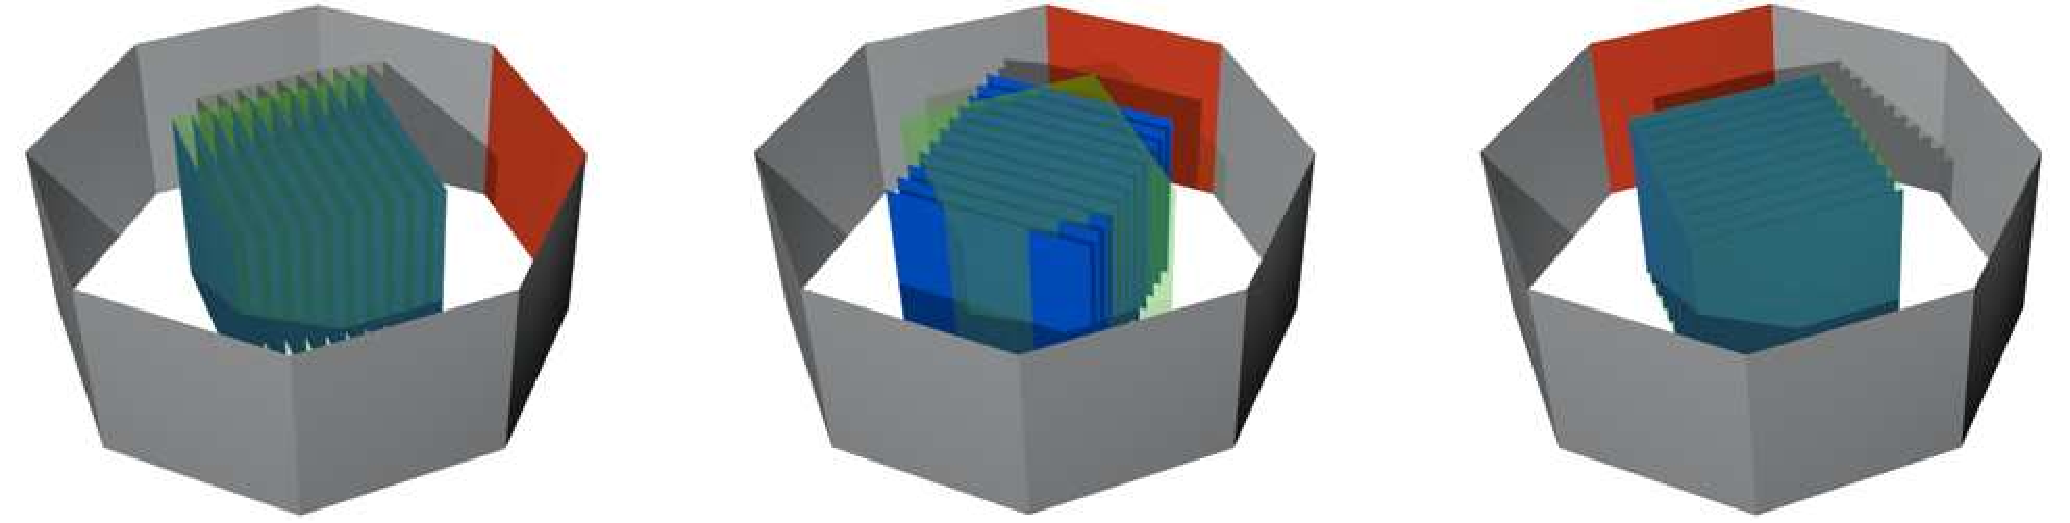
\includegraphics[width=4.3in]{gpu_3}
\caption{Rotation-based projection: the activity is re-sampled on a regular grid aligned with a camera and then projected. 
This enables FFT based convolution with the (depth-dependent) collimator-detector response.}
\label{fig:rotation}
\end{figure}

Let the radio-pharmaceutical activity within the region of interest of the patient's body be a continuous function 
denoted by $\tilde{y}$. 
In order to readily discretize the reconstruction algorithm, it is convenient to imagine that the activity is in first place 
discrete in space \cite{shepp_1982}. 
Let us approximate $\tilde{y}$ by a set of point sources $y=y_{b}, b=1,..,N_{b}$ displaced on a regular grid.

\noindent As each point source emits radiation at an average rate $y_{b}$ proportional to the local density of radio-tracer 
and emission events in a same voxel are not time correlated, the number of emissions in the unit time is a Poisson 
distribution of expected value $y_{b}$. The geometry of the system and attenuation in the patient 
determine the probability $p_{bd}$ that a photon emitted in $b$ is detected at detector pixel $d$.
From the sum property of the Poisson distribution, the photon count in $d$ has Poisson \textit{pdf} 
with expected value $\sum_{b}p_{bd}y_{b}$. 
Given activity $y$, the probability to observe counts $z$ is 


\begin{equation}
 \label{eq:pzy}
 p(z|y) = \prod_{d=1}^{N_{d}}{\mathcal{P}(\sum_{b}p_{bd}y_{b}, z_d)}
\end{equation}

\noindent Amongst all the activity configurations that might have generated the observed photons, 
the activity that maximizes the \textit{likelihood} function is optimal 
in the sense of the L2 norm of the difference from the true value, for the log linear distribution $p(z|y)$ \cite{cramer_1957}.

\begin{equation}
 \label{eq:y}
 \hat{y} = \arg\max_y\ p(z|y) = \arg\max_y\ \log{p(z|y)}
\end{equation}

\noindent Expanding $log{\ p(z|y)}$:

\begin{equation}
 \label{eq:y2}
 \hat{y} = \arg\max_y\ \sum_{d=1}^{N_{d}}\left( \sum_{b}p_{bd}y_{b} + z_{d} \log\sum_{b}p_{bd}y_{b}\right)
\end{equation}

\noindent A gradient-based optimization algorithm, such as gradient ascent, requires the gradient of the likelihood function 
with respect of the activity in each point source, differentiating the log of \ref{eq:pzy}:

\begin{equation}
 \label{eq:pro}
 \frac{\partial \log p(z|y)}{\partial y_{r}}\vert_{y=\bar{y}} = \sum_{d=1}{p_{bd}} + \sum_{d=1}p_{bd}{\frac{z_d}{ \sum_{b^{\prime}}p_{b^{\prime}d}\ y_{b^{\prime}} }}\vert_{y=\bar{y}}
\end{equation}

\noindent $\sum_{b^{\prime}}p_{b^{\prime}d}\ y_{b^{\prime}}$ is referred to as projector, and $\sum_{d}{p_{bd}f_d}$ as backprojector of $f_d$.

\noindent Similarly the Expectation Maximization algorithm for maximization of the \textit{likelihood} (MLEM) 
implies projection and backprojection \cite{shepp_1982}:

\begin{equation}
 \label{eq:mlem}
 \hat{y}_b^{(k+1)} = \hat{y}_b^{(k)} \frac{1}{\sum_{d}{p_{bd}}} \sum_{d}{p_{bd}\frac{z_d}{\sum_{b^{\prime}}p_{b^{\prime}d}\ \hat{y}^{(k)}_{b^{\prime}}}}
\end{equation}

\noindent In case of ideal CDR, with a parallel hole collimator, the system matrix $p_{bd}$ is non-zero only along 
lines perpendicular to the collimator entry surface and the 
projection is a line integral operator. A more detailed system model accounts for the sensitivity 
of each detector pixel to radiation emissions from each voxel. With a planar detector, coupled to a parallel hole, cone beam or fan beam collimator, 
the sensitivity is invariant to shift along the detector plane. With shift invariant CDR, 
projection is factorisable into a line integral operator and a convolution operator \cite{zeng_1992}. 
The CDR is generally dependent upon the distance from the detector plane. \\

The rotation-based projection and backprojection algorithm proposed by Zeng and Gullberg \cite{zeng_1992} was adopted
as it suits the GPU architecture and is convenient to be incorporated with depth-dependent response functions. 
For each position of the gamma camera, the image matrix volume is rotated so that the front face of the volume faces the 
detection plane - Figure \ref{fig:rotation}. As the image is re-interpolated on a grid that is aligned with the detection plane, all the point sources that lay on a same 
plane parallel to the detector are now at the same distance from the detector. A depth-dependent PSF that models the 
CDR can be incorporated efficiently by convolving each parallel plane with the PSF that models the 
relative to the distance of the plane from the collimator. 
The convolution can be performed by multiplication in the frequency domain, reducing the complexity from $O(N^2)$ to $O(N \ logN)$. 

\noindent Backprojection similarly takes advantage of rotation to incorporate the depth dependent PSF. Details of the implementation of the projector 
and backprojector are given in the next section.

\subsection{GPU acceleration}
\begin{figure}[h]
\centering
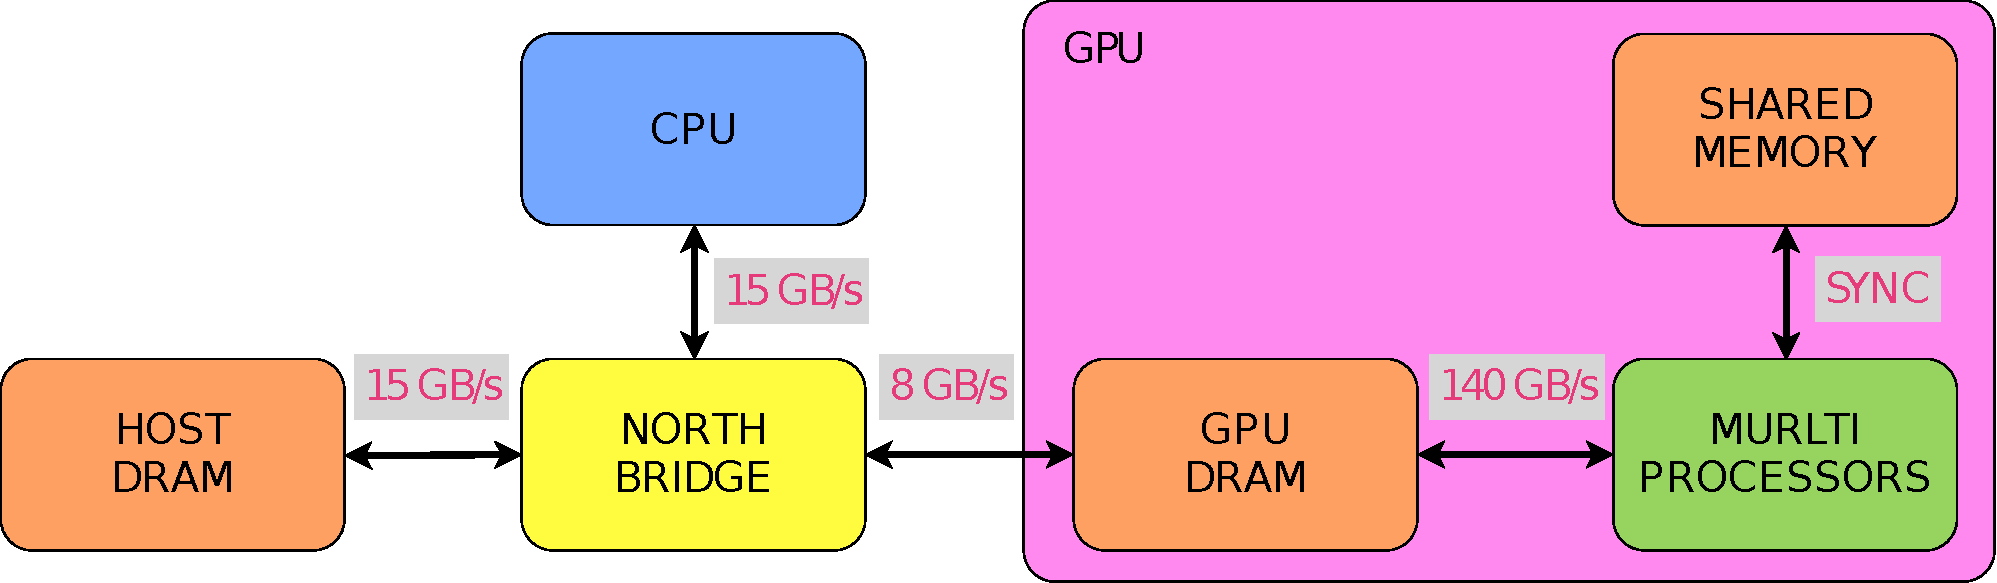
\includegraphics[width=4.3in]{gpu_6}
\caption{Memory structure of the host machine and GPU and typical memory bandwidth.}
\label{fig:hardware}
\end{figure}

For problems that present enough task parallelism, state of the art GPUs can provide an acceleration of up to 10x over a high end CPU, 
however the speedup can increase by another order of magnitude if the structure of the algorithm allows for efficient 
use of the \textit{shared memory} of the GPU \cite{stone_2007, ufimtsev_2008, pedemonte_2009}.  
While on CPUs the cache hierarchy compensates costly accesses to external RAM 
and cache heuristics account for a large class of computational problems, the simplified memory hierarchy 
of GPUs requires careful design of the algorithms for efficient memory access. The external memory is directly exposed to the programmer, 
who has to consider explicitly coalesced access due to the mismatch between data rate and cycle time of the DDR memory. On the other hand 
the simpler structure of the memory and vicinity of the RAM to the processor yield data throughput 10 times higher than the 
throughput between CPU and RAM - Figure \ref{fig:hardware}. \\

The fast RAM memory of the GPUs explains the $10\times$ speedup, however the Single Instruction Multiple Data (SIMD) architecture and the 
\textit{shared memory} of the GPU provide additional speedup for a class of computational problems. In the SIMD architecture, 
many processor cores fit on the same chip due to simplified design of the processor cores, 
which are grouped, in the case of NVidia GPUs, in a \textit{multiprocessor} with a single common fetch unit. Multiple 
cores can operate concurrently in a \textit{multiprocessor} if they execute the same instruction, so 
if the computational problem is such that the same operation is performed on multiple segments of data, the GPU 
can use a great number of processors at the same time. As the RAM data throughput would still be too low to continuously feed data to all 
the cores, the processor cores that are grouped in a \textit{multiprocessor} have access to an on-chip memory that can be read and written 
concurrently by all the cores in a single clock cycle, through multiple data paths. The size of the \textit{shared memory} is limited to a few 
Kbytes on currently available GPUs. This design offers the possibility to exploit the full power of the cores as long as the cores 
in a multiprocessor can reuse the data that resides in the \textit{shared memory}, hiding accesses to the global memory, that is hundreds of times slower. 
In order to take full advantage of the GPU architecture, a computational problem needs to expose parallel tasks that run on each multiprocessor, 
each task being partition-able into serial tasks that use limited memory (up to a few Kbytes) and present a high ratio 
between the number of operations and the accesses to memory.\\

Another feature offered by Nvidia GPUs is hardware trilinear interpolation. A portion of memory may be specified as a 1D, 2D or 3D array and floating 
point memory addresses are accepted by the memory access unit, which decodes the non-integer address, reads the values stored in the nearest 
memory locations and interpolates linearly. \\

\begin{figure*}[h]
\centering
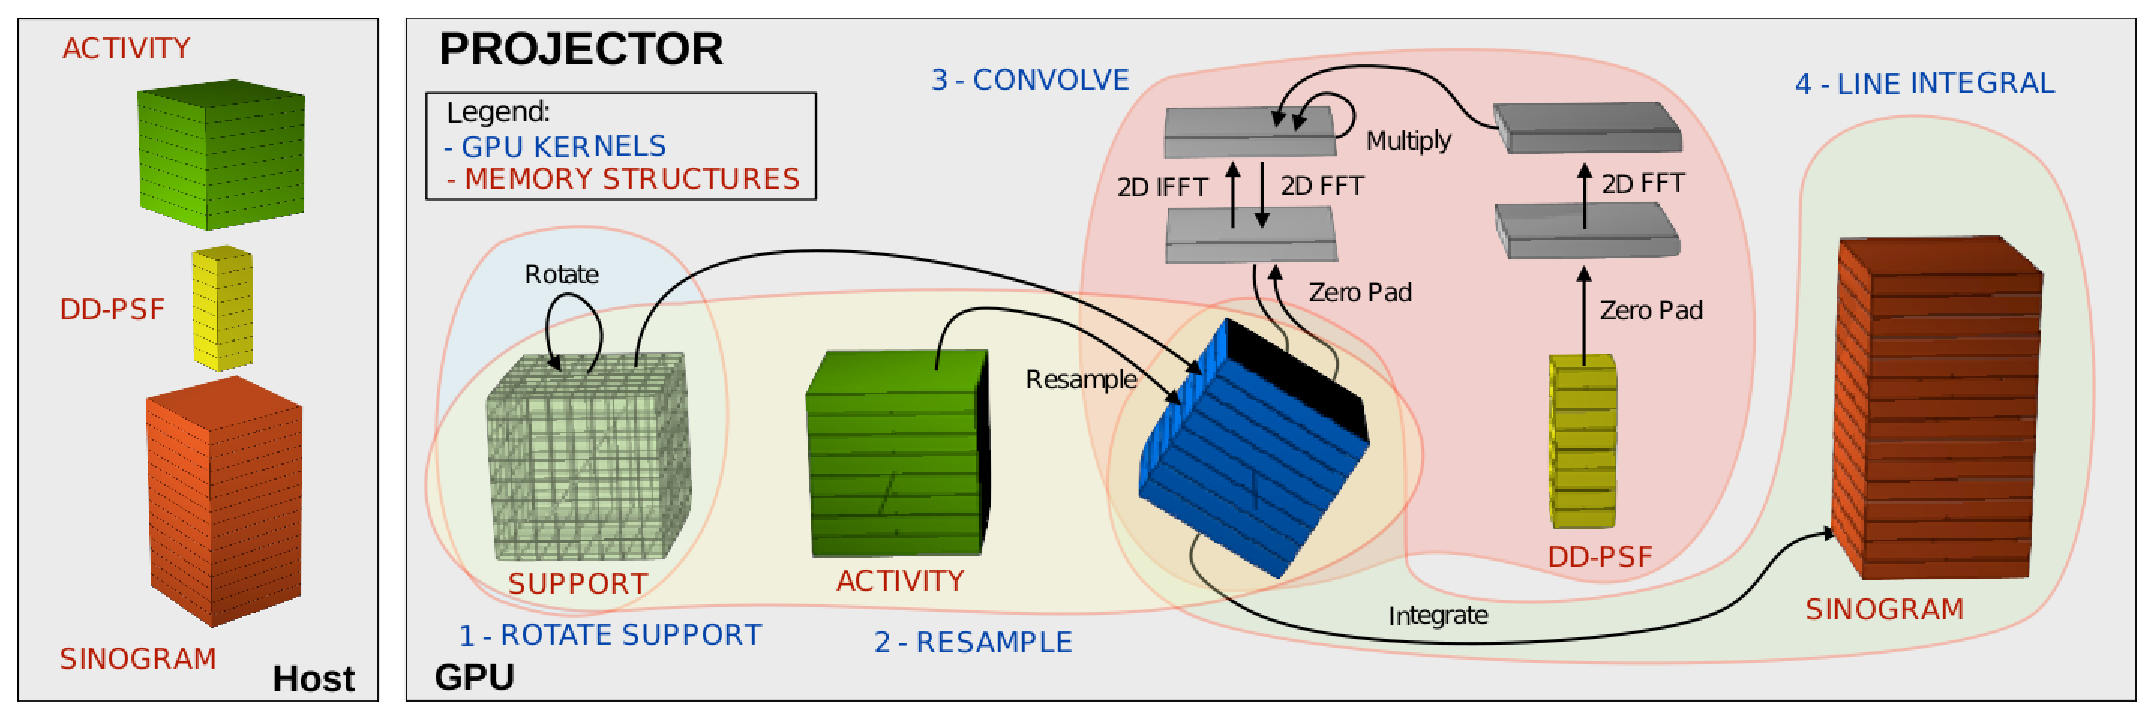
\includegraphics[width=4.3in]{gpu_1}
\caption{Rotation-based projection on GPU}
\label{fig:gpu_projection}
\end{figure*}

Ray-tracing on GPU can take advantage of the fast RAM memory of the GPU and of hardware interpolation, 
however independence of the rays impedes efficient use of the \textit{shared memory}. It might be possible to 
take advantage of the shared memory as the rays share some information, however that would imply processing 
concurrently multiple partial rays in blocks in a way that exposes the data in common. 
Rotation-based projection and backprojection reorganize data in a way that exposes the data locality. \\

\vspace{3mm}
\subsubsection{Projector}
Activity and the depth dependent PSF are copied to the GPU global memory and additional memory is allocated for the sinogram and 
for each of the structures depicted in Figure \ref{fig:gpu_projection}. 
The support of the image (ordered list of the $x,y,z$ indexes of the image voxels) is extracted and stored in global memory. \\

\begin{figure*}[h]
\centering
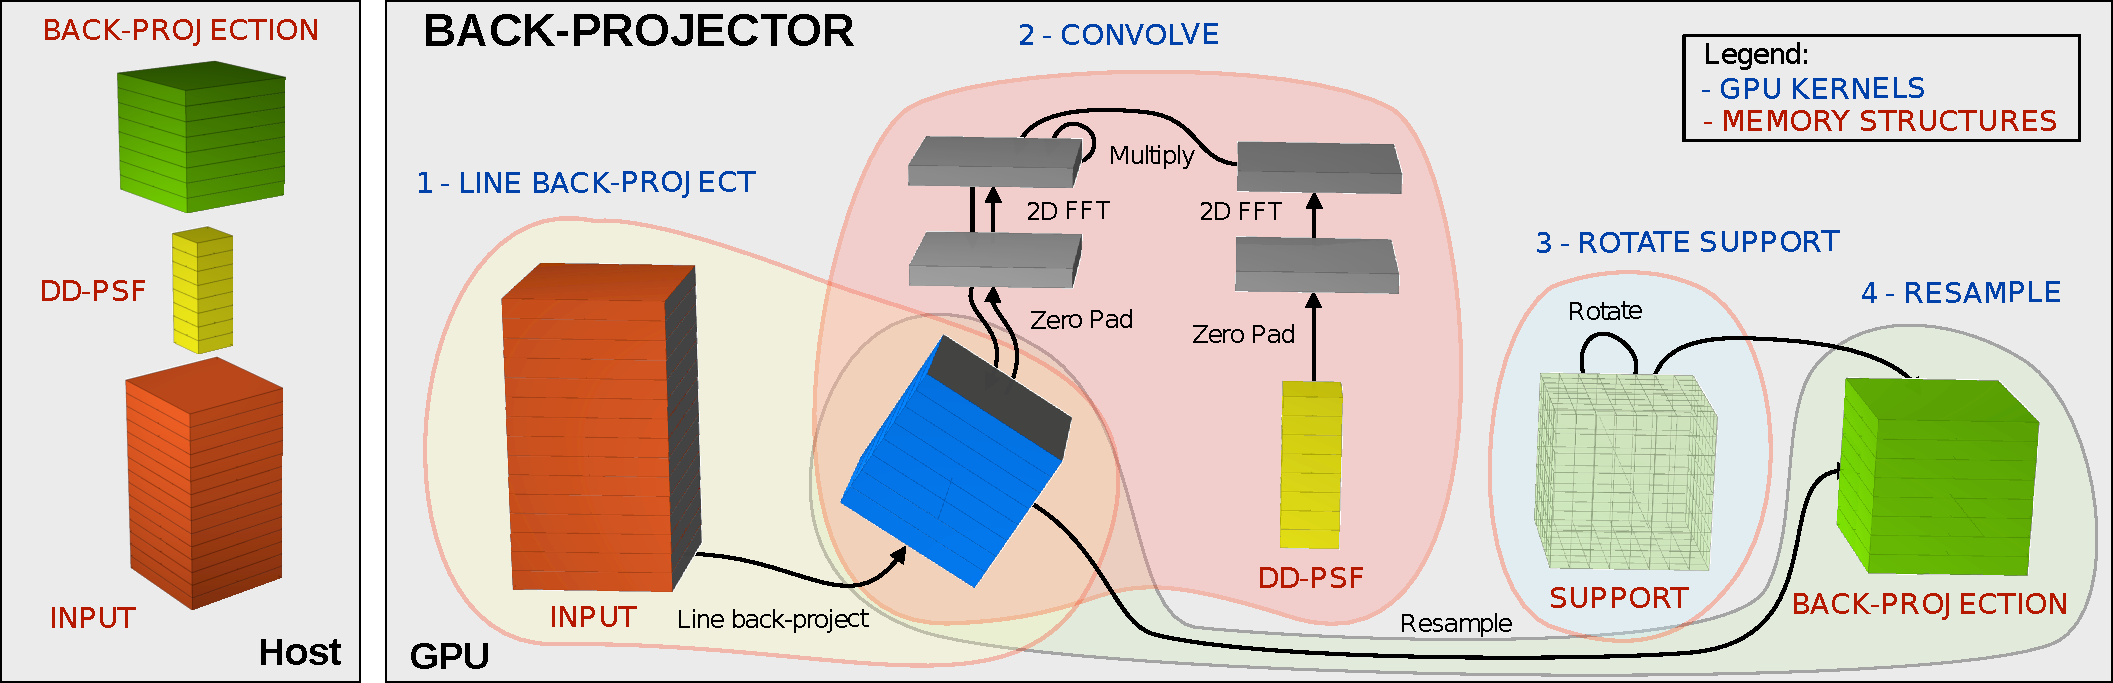
\includegraphics[width=4.2in]{gpu_4}
\caption{Rotation-based backprojection on GPU}
\label{fig:gpu_backprojection}
\end{figure*}

\noindent For each position of the gamma camera, the activity matrix volume is rotated so that the front face of the volume faces the 
detection plane. In order to optimize the usage of the GPU, rotation is performed by multiplying the support of the image 
by the rotation matrix, then the image is re-sampled at the locations specified by the rotated support. Rotation of the support 
maximizes the \textit{device occupancy} (concurrent usage of the multiprocessors) and takes advantage of the \textit{shared memory} 
by partitioning the matrix multiplication \cite{cuda}. The trilinear interpolation is performed in hardware by the \textit{texture fetch} unit 
of the GPU at the cost of a memory access and coalesced memory accesses are obtained by partitioning the memory transfers in blocks.\\
 
\noindent For each camera's position, the activity is rotated from its initial position, rather than from the previous camera's position, in 
order to minimize interpolation errors. After reinterpolation, each image plane parallel to the camera is convolved with the PSF. 
Convolution is performed by zero-padding the plane to double its linear size, computing its 2D FFT, multiplying by 
the FFT of the zero-padded PSF, back-transforming and truncating. As depicted by the arrows in Figure \ref{fig:gpu_projection}, the 
convolution is performed in place, in order to minimize memory occupancy. 2D FFT is performed by means of the CUDA CUFFT library that takes into account 
all the architectural factors and constraints of CUDA, memory coalesced access, bank conflicts and efficient shared memory usage. \\

\noindent Finally a kernel sums all planes and stores the result in the sinogram data structure. Shared memory cannot be used in the summation step 
as the number of operations (sums) is exactly equal to the number of memory accesses, 
however \textit{device occupancy} and memory coalescing are optimized by partitioning the sums in blocks. \\


\vspace{3mm}
\subsubsection{Backrojector}
The sinogram and the PSF are transfered from the host machine RAM to the GPU global memory and all the structures depicted in 
Figure \ref{fig:gpu_backprojection} are allocated on the GPU memory. Two volumes are allocated for the backprojection, a rotating 
volume and a fixed volume that is initialized to $0$ and contains in the end the result of the backprojection.\\

\noindent One projection at a time is extracted from the sinogram data structure and the value on each pixel is backprojected to 
the rotating volume along lines perpendicular to the detection plane. This step is performed by a GPU \textit{kernel} 
that copies a pixel to a local \textit{register} and then copies it back into all the voxels in the same column of the rotating volume. 
Each plane of the rotating volume is then convolved in place with the PSF by multiplication in the frequency domain. 
The rotating volume is rotated to the zero position and then accumulated into the fixed volume. \\

\noindent The same series of operations is repeated for each camera's position.


\subsection{Reconstruction Algorithms}
On top of the projection and backprojection routines, NiftyRec implements a number of reconstruction algorithms. 
Let the radio-pharmaceutical activity within the region of interest of the patient's body be 
denoted by $y_b$ with $b=1,..,N_b$ and the number of counts in a detector bin be denoted by $n_d$, with $d=1,..,N_d$. The probability that a photon emitted 
in $b$ is detected in $d$ is denoted by $p_{bd}$.

\subsubsection{MLEM}
Maximum Likelihood Expectation Maximization \cite{shepp_1982}.

\begin{equation}
 \hat{y}_b^{(k+1)} = \hat{y}_b^{(k)} \frac{1}{\sum_{d}{p_{bd}}} \sum_{d}{p_{bd}\frac{z_d}{\sum_{b^{\prime}}p_{b^{\prime}d}\ \hat{y}^{(k)}_{b^{\prime}}}}
\end{equation}

\noindent where $k$ is the itaration number. Unconstrained MLEM suffers from dimensional instability: after a certain number of iterations the noise starts 
to diverge; for this reason typically the algorithm is stopped after a given number of iterations. Maximum a-posteriori reconstruction algorithms can converge 
to a global maximum and thus can easily adopt stopping criteria based on relative error of the image estimate. 

\subsubsection{OSEM}
Ordered Subsets Expectation Maximization \cite{hudson_1994}: projection data is divided into an ordered sequence of subsets. An iteration of OSEM is defined as a single pass
through all the subsets, in each subset using the current estimate to initialize application of EM with that data subset. 
In SPECT the OSEM algorithm can provide more than an order of magnitude acceleration over MLEM, maintaining similar image characteristics. 
While any subset of the projection space may be considered, here by subset we intend a subset of the projection angles. 

\begin{equation}
 \hat{y}_b^{(k)}(i+1) = \hat{y}_b^{(k)}(i) \frac{1}{\sum_{d\in S(i)}{p_{bd}}} \sum_{d\in S(i)}{p_{bd}\frac{z_d}{\sum_{b^{\prime}}p_{b^{\prime}d}\ \hat{y}^{(k)}_{b^{\prime}}(i)}}
\end{equation}

\noindent where $\hat{y}_b^{(k)}(i+1)$ represents the updated iterand after processing subset $i$, $S(i)$ contains the projection angles of subset $i$ and $k$ represents the iteration number. 

\subsubsection{OSL-MAPEM}
Maximum a-posteriori Expectation Maximization does not generally have a closed form solution, however the One Step Late (OSL) algorithm 
introduced by Green \cite{Green} can be adopted with any prior that is differentiable once with respect to the activity in each voxel $b$. 

\begin{equation}
 \hat{y}_b^{(k+1)} = \hat{y}_b^{(k)} \frac{1}{\sum_{d}{p_{bd}} - \frac{\partial{p(y)}}{\partial{y_b}}\vert_{y=\hat{y}^{(k)}}} \sum_{d}{p_{bd}\frac{z_d}{\sum_{b^{\prime}}p_{b^{\prime}d}\ \hat{y}^{(k)}_{b^{\prime}}}}
\end{equation}

\noindent where $p(y)$ is the prior probability of activity $y$. The Matlab Toolbox of NiftyRec has a few examples of activity priors, such as Total Variation and priors 
based on a coregistered intra-subject anatomical image. Please refer to the inline Matlab documentation. 

\subsubsection{Gradient Ascent}
NiftyRec implements a simple gradient ascent algorithm for optimization of the log likelihood and log posterior for maximum a-posteriori estimation of the activity. 

\begin{equation}
 \log p(y|z)\ \alpha\ \log p(z|y) + \log p(y)
\end{equation}

\begin{equation}
 \hat{y}^{(k+1)} = \hat{y}^{(k)} + \beta \left(\frac{\partial\log p(z|y)}{\partial y_{r}}\vert_{y=\hat{y}^{(k)}} + \frac{\partial\log p(y)}{\partial y_{r}}\vert_{y=\hat{y}^{(k)}} \right)
\end{equation}

\begin{equation}
 \frac{\partial \log p(z|y)}{\partial y_{r}}\vert_{y=\bar{y}} = \sum_{d=1}{p_{bd}} + \sum_{d=1}p_{bd}{\frac{z_d}{ \sum_{b^{\prime}}p_{b^{\prime}d}\ \hat{y}^{(k)}_{b^{\prime}} }}
\end{equation}

The Matlab Toolbox of
NiftyRec has a few examples of activity priors, such as Total Variation and
priors based on a coregistered intra-subject anatomical image. Please refer
to the inline Matlab documentation.

\subsubsection{Scatter correction}
NiftyRec implements the Reconstruction Based Scatter Compenstation (RBSC) algorithm for scatter compensation \cite{kadrmas_1998}.

\begin{equation}
 \hat{y}_b^{(k+1)} = \hat{y}_b^{(k)} \frac{1}{\sum_{d}{p_{bd}}} \sum_{d}{p_{bd}\frac{z_d}{\sum_{b^{\prime}}p_{b^{\prime}d}\ \hat{y}^{(k)}_{b^{\prime}} + \hat{n_d}^{SC} }}
\end{equation}

%%=================================================================================
%%Developer Guide


\chapter{Developer's Guide}

\section{Getting Started}
The Developer's Guide is intended for those who want to extend the functionality of NiftiRec; 
it explains the algorithms that NiftyRec implements, outlines the structure of the code and explains 
how to extend it. Please refer to the User's Guide in order to use NiftyRec through the C API or the Python or Matlab interfaces. 
In this case you will not need to understand all the bits and pieces of NiftyRec. \\

In order to embed NiftyRec functionalities within third party applications or to cerate custom applications 
that make use of NiftyRec through its C API, it is not necessary to build NiftyRec from the source if a Packaged 
Release \ref{sec:packaged_release} is available for the architecture and operating system of your machine. 
In this case, you might want to simply link against the NiftiRec compiled libraries. All the NiftiRec 
libraries and header files are installed by the self installer of the Packaged Release. A CMake FindPackage 
module is provided \ref{sec:directory_tree} in order to find automatically the headers and libraries with CMake.\\

If you intend to extend NiftiRec then you will have to compile it from source. Compilation is based on the 
cross-platform build-system CMake.\\

%\subsection{Download Source Code}
%NiftiRec is freely downloadable from Sourceforge and completely open source: \url{http://niftk.sourceforge.com}\\

\subsection{Compile with CMake}
NiftyRec is based on the CMake cross-platform build-system.  
Compilation of NiftyRec with CMake generates all the libraries, the binary executable files and the documentation, 
and optionally creates a self-installing package for your platform for distribution of NiftyRec binaries. 
The self-installing package will install all the libraries, the binary executables, the documentation,  
the development file headers and the Matlab and Python toolboxes. Self-installers for some of the most 
common platforms can be downloaded from \url{http://niftk.sourceforge.com}.
In order to extend the functionality of NiftyRec it is necessary to download its source and compile 
with CMake. 

\subsubsection{Linux Debian}
\noindent Install ccmake or cmake-gui. Under Debian Linux install from repositories: \\
   
   \emph {..\$ sudo apt-get install cmake-gui}\\

\noindent Download and uncompress NiftyRec source. cd to the 
   project main directory, create here a folder 'build', cd to that folder 
   and run cmake: \\

   \emph {..\$ mkdir build}\\
\indent   \emph {..\$ cd build}\\
\indent   \emph {..\$ cmake-gui ..}\\

\noindent    Select options, set the BUILD\_TYPE to Release or to Debug and set all the required 
   paths for additional dependencies if you selected any of the options. 
   Configure and Generate. Now quit ccmake/cmake-gui and build\\
  
   \emph {..\$ make build}\\

\noindent    In order to create an installation package with CPack run make with option 'package'\\

   \emph {..\$ make package}\\

\noindent    In order to install NiftyRec in the system run make with option 'install'\\

   \emph {..\$ sudo make install}\\

\noindent    or install the package created with 'make package'.

\subsubsection{Windows}
Install cmake. Download and uncompress source. Open the source directory 
with Windows Explorer and create here a new folder 'build'. Launch CMake 
and open CMakeLists.txt from the main directory of NiftyRec.
Select options, set the BUILD\_TYPE to Release or to Debug and set all the required 
paths for additional dependencies if you selected any of the options. 
Configure and Generate. Browse the 'build' directory and double click 
on the Visual Studio project file. Click Compile button in Visual Studio. 
Create self-extracting installer by compiling the corresponding target in Visual 
Studio. 
%\subsubsection{Mac OS}

\section{Software Overview}

\subsection{Directory Tree}
\label{sec:directory_tree}

\definecolor{gray}{rgb}{0.5,0.5,0.5} 
\dirtree{%
.1 /. 
.2 \textcolor{gray}{CMakeLists.txt} \DTcomment{\begin{minipage}[t]{7cm} 
                  Main CMake list file, sets up build options and includes all the subfolders.
                  \end{minipage}}. 
.2 et-lib         \DTcomment{\begin{minipage}[t]{7cm} 
                  Source code of NiftyRec core libraries. All of NiftyRec libraries are here except for the mex extensions and the GPU accelerated routines, which are in  
                  et-lib\_gpu.
                  \end{minipage}}.  
.3 \textcolor{gray}{\_et.cpp.txt}            \DTcomment{\begin{minipage}[t]{7cm}
                                             Implements the Nifti Interface. The subset of the NiftyRec functions defined here allows to use all the functionalities of NiftyRec. 
                                             The C Array Interface only imports this library, which binds to all other libraries of NiftyRec, including the libraries 
                                             for GPU acceleration. 
                                             \end{minipage}}. 
.3 \textcolor{gray}{\_et\_array\_interface.cpp} \DTcomment{\begin{minipage}[t]{7cm}
                                             Implements the C Array Interface. 
                                             \end{minipage}}. 
.2 et-lib\_gpu    \DTcomment{\begin{minipage}[t]{7cm}
                  Routines for GPU acceleration. They are functinoally identical to some of the functions in et-lib but these make use of the NVidia CUDA Runtime interface 
                  for GPU acceleration. 
                  \end{minipage}}. 
.2 et-mex         \DTcomment{\begin{minipage}[t]{7cm}
                  Contains the source code for the Matlab extensions. Each Matlab extension function has a .cpp and a .h file. 
                  The Matlab Toolbox is made up of mex extensions, m files and documentation. Subfolders of et-mex contain the m files 
                  and the Documentation. 
                  \end{minipage}}. 
.3 m                                         \DTcomment{\begin{minipage}[t]{7cm}
                                             m files for the Matlab Toolbox.
                                             \end{minipage}}. 
.3 doc                                       \DTcomment{\begin{minipage}[t]{7cm}
                                             Documentation for the Matlab Toolbox.
                                             \end{minipage}}. 
.2 NiftyRec       \DTcomment{\begin{minipage}[t]{7cm}
                  Python extension module.
                  \end{minipage}}. 
.2 et-apps        \DTcomment{\begin{minipage}[t]{7cm}
                  Standalone applications based on NiftyRec
                  \end{minipage}}. 
.2 et-doc         \DTcomment{\begin{minipage}[t]{7cm}
                  NiftyRec documentation.
                  \end{minipage}}. 
%.2 images         \DTcomment{\begin{minipage}[t]{7cm}
%                  Images.
%                  \end{minipage}}. 
%.2 misc           \DTcomment{\begin{minipage}[t]{7cm}
%                  Miscellaneous functions not directly related to NiftyRec.
%                  \end{minipage}}. 
}


%\subsection{Data Structures}

\subsection{Programming Guidelines}
Development of NiftyRec is inspired to the agile programmiong philosophy, Working software is the principal 
measure of progress, face-to-face conversation between the developers has been the main form of communication. 
There was a continuous attention to good design and technical excellence, while always opting for 
simplicity. The programmers tried to make the code as open as they could by adopting meaningful names, following consistent naming 
conventions and avoiding criptic bits of code. 
As in Unix Programming, data dominates, the code is based on the data structures defined in the niftilic \url{http://niftilib.sourceforge.net/} 
library and given this choice the algorithms are almost self-evident.

%\subsection{Programming Interfaces}


\section{Programming Interfaces}

  \begin{figure}[htbp]
    \label{fig:api}
    \begin{center}
      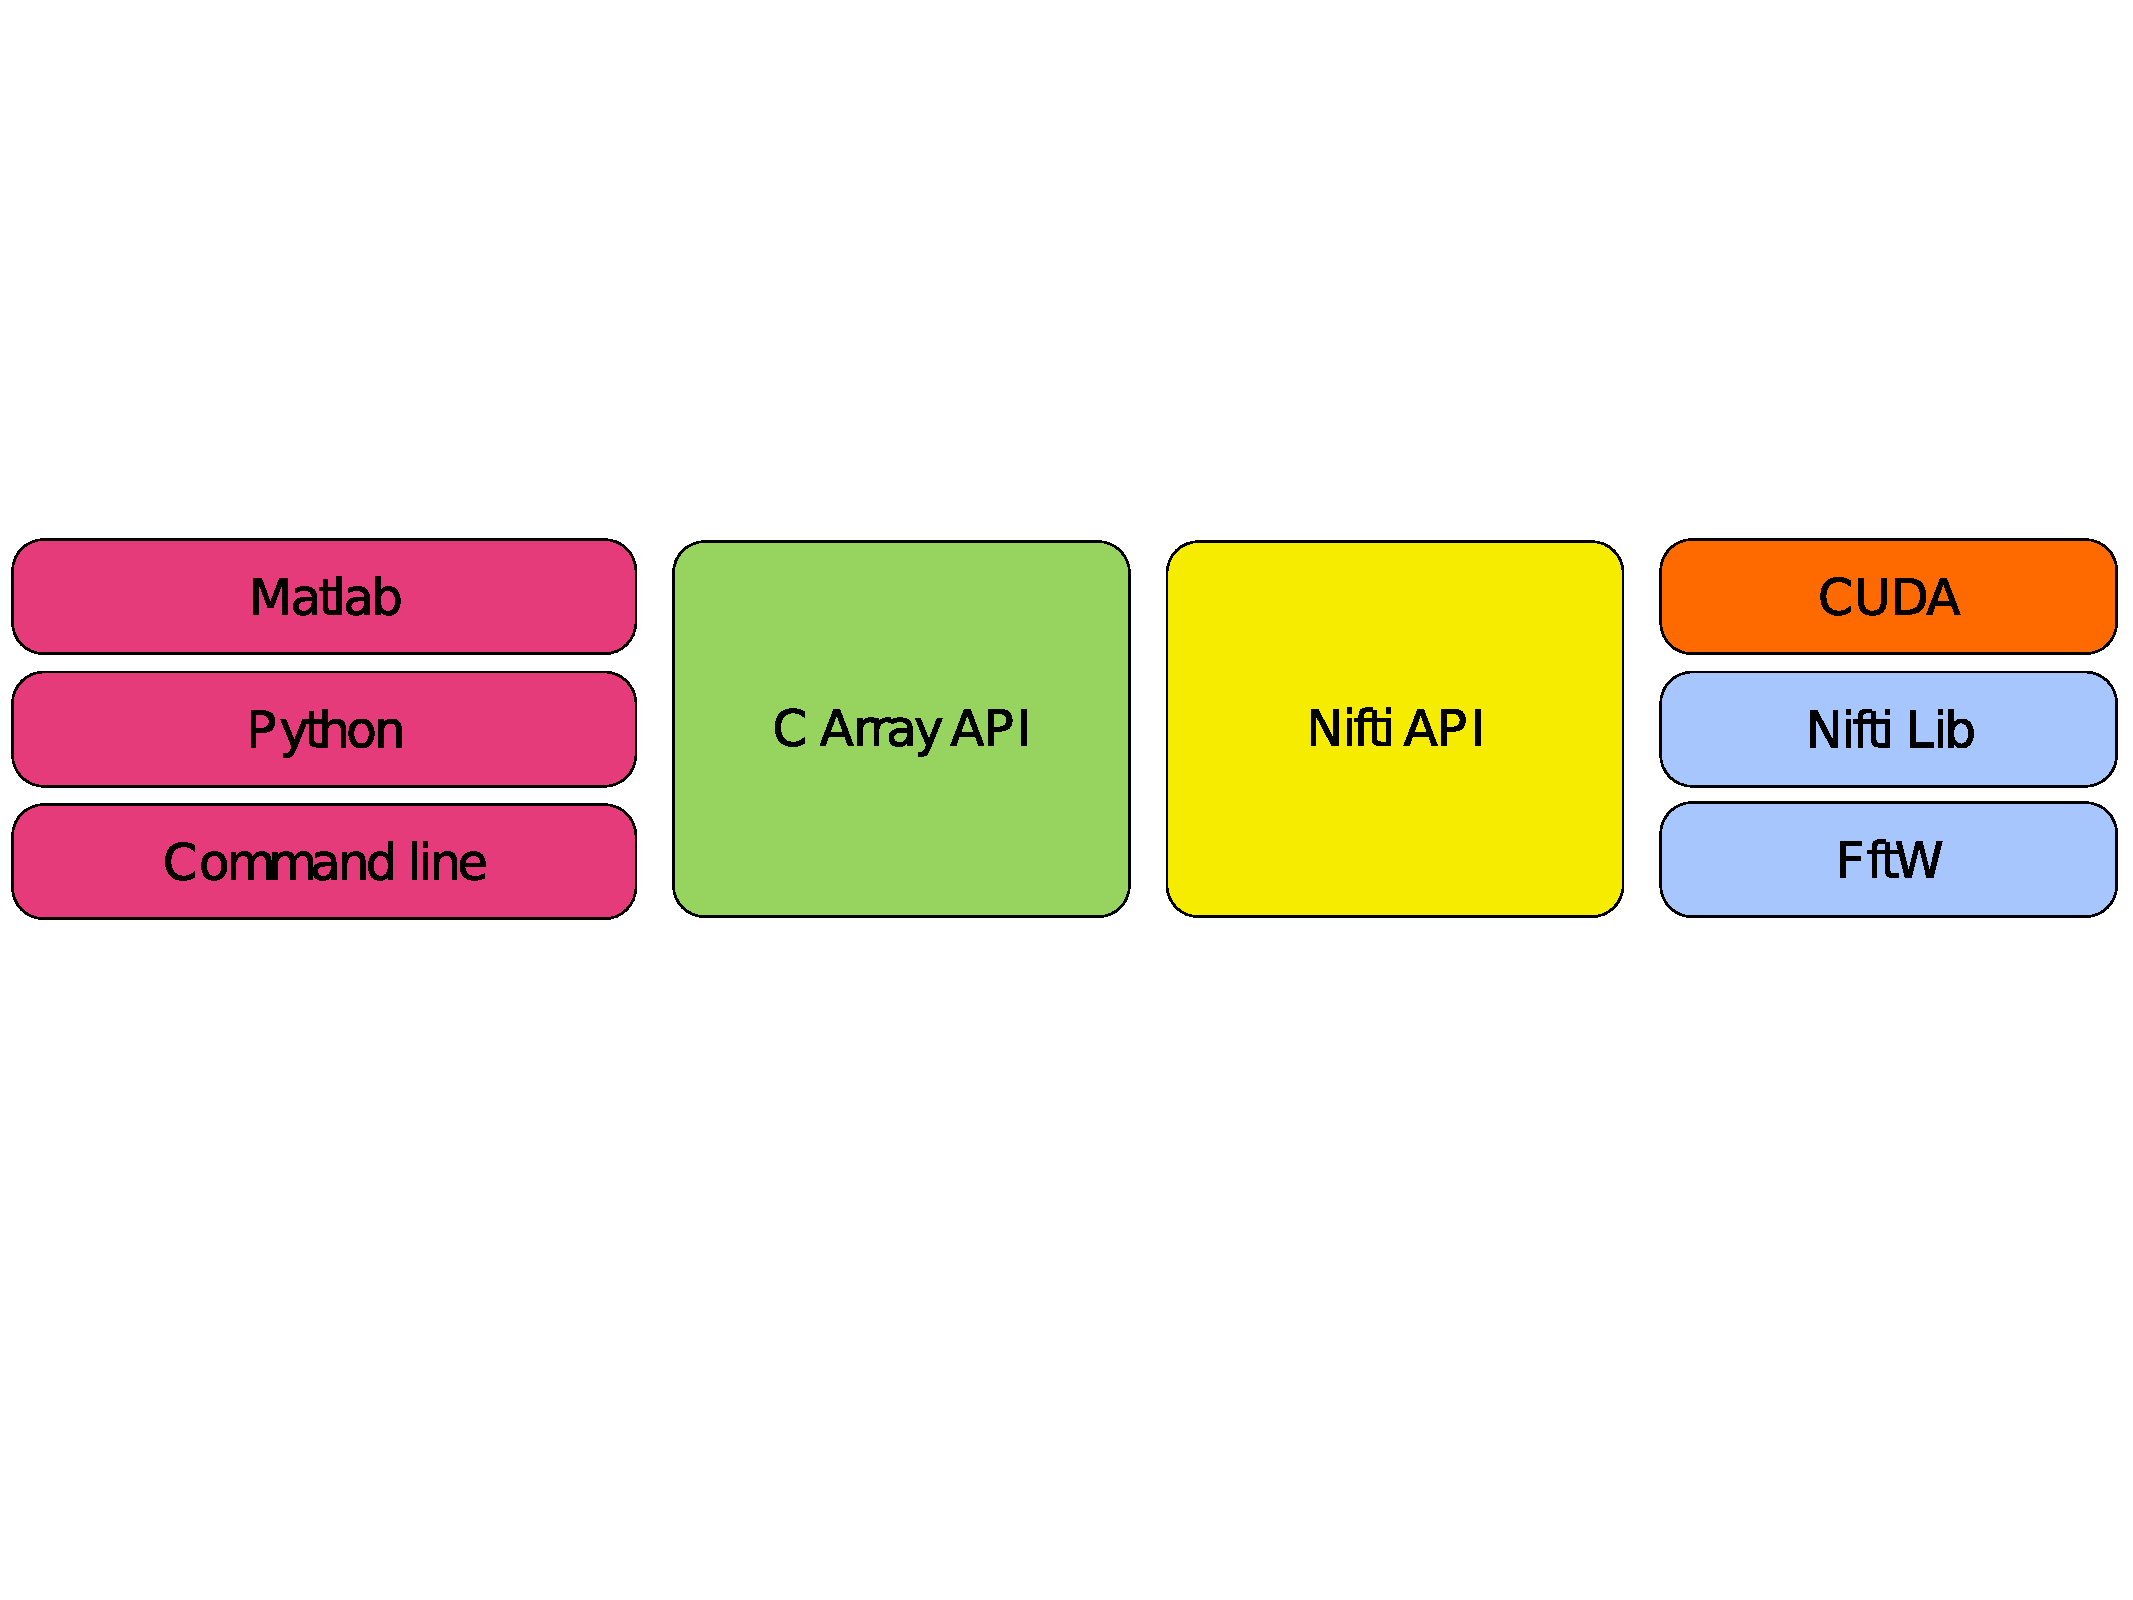
\includegraphics[width=4.3in]{api}
    \end{center}
  \end{figure}

\subsection{Nifti Interface}
All functions in NiftyRec take as parameters pointers to \emph{nifti\_image} data structures, defined in \emph{niftilib}. 
Developing NiftyRec is simple, one needs to understand what are the fields in the \emph{nifti\_image} structure. 
These structures are well suited to medical images and image in general (in a broad sense, activity, projections, gradients, 
attenuation image, point spread function, ..) as all the parameters of interest for the image are 
stored in the structure, allowing one to pass the image and all the information relevant to that image, by one pointer. 
NiftyRec makes heavy use of \emph{nifti\_image} structures, most of the functions take as parameters pointers to \emph{nifti\_image} 
structures which they can then read and modify. 

\subsection{C Array Interface}
While NiftyRec internally uses the \emph{niftilib} data structures in order to simplify the handling of images and parameters, 
it provides a programming interface entirely based on C arrays in order to simplify embedding of NiftyRec into third party applications. 
The programmer who wants to make use of NiftyRec but does not intend to extend its functinoality, shouldn't 
be required to learn how to use the niftilib data structures (though they are quite simple). The C Array Interface is based entirely on 
C arrays and exposes a subset of the functions of NiftyRec that allows one to use all its functionalities. \\

The source files \emph{et-lib/\_et\_array\_interface.cpp} and \emph{et-lib/\_et\_array\_interface.h} implement the C Array Interface. 
Each of the functions defined here assembles the required niftilib structures, calls a function from the Nifti Interface, then destroys the structures that 
it created. \\

Note that Matlab and Python bindings are built on top of the C Array Interface, as pictured in figure \ref{fig:api}.

\subsection{Matlab}
The Matlab Toolbox for NiftyRec is based on mex Matlab extensions. 
Each of the functions of the NiftyRec C Array Interface has a corresponding mex source file that 
defines its interface to Matlab. The folder \emph{et-mex} contains the source code of the mex extensions. 
Subfolders of \emph{et-mex} contain additional Matlab m files and the Matlab inline documentation and manual for NiftyRec.
The mex interface is a thin layer on top of the C Array Interface. Each function correponds to one .cpp source file and a .h header 
in \emph{et-mex}. Edit one of the mex sources in \emph{et-mex} to understand how to create a mex extension for a new function in the C Array Interface.\\

Note that often mex Matlab extensions are compiled within Matlab by running the \emph{mex ..} command with the source files as parameters. This creates a mex file, which 
Matlab recognises as an extension. The mex file is actually a shared library (where the extension of the file is renamed); Matlab uses an external compiler to generate the mex 
and it sets up automatically all the options for the compiler, including where it can find the Matlab libraries (which the mex file builds against). NiftyRec uses the compiler 
directly to build the mex. A macro in the CMake list file (\emph{et-mex/CMakeLists.txt}) sets the parameters for the compiler and edits the extension of the output dynamic libraries. This allows us to automatically compile the Matlab extensions along with the NiftyRec source.


\subsection{Python}
Python bindings are built on top of the C Array Interface and are based on Python Ctypes. 
Ctypes is a Python module that allows one to interface dynamic libraries written in C and 
execute functions that make use of basic C types such as int, float, double, char, arrays and pointers to the 
former types. There are a few advantages of Ctypes over other methods to interface C code with Python, one being simplicity of 
use and another being that the interface is independent from the version of Python and from the compiler. 
Building a Python extension module against the Python libraries defined in Python.h requires the same compiler that 
was used to compile the Python libraries; this is generally not a problem under Linux, but it can be a problem 
under Windows, where Python is typically installed with the self-extracting installer which adds to the system a 
copy of the libraries that was compiled with a specific compiler, which typically is a commercial compiler. 
The same problem applies to all the automatic wrappers that create code to be built againsts Python libraries. 
Ctypes however is a good solution as long as the number of functions to be wrapped is small and as long as is suffices 
(or is not over complicated) to use only basic C types, which is the case of NiftyRec.\\

If you edit \emph{et\_array\_interface.cpp} you will notice that all the functions that are exposed to Python are defined with 
the \emph{extern "C"} syntax in order to instruct the compiler to treat them as C functions. This solves the 
problem of using C++ code through Ctypes because of mangling of the function names for overclassing: C++ compilers modify 
the function names in order to encode the types of the parameters for that particular implementation of the function, though 
the compiler changes the name in a predictable manner, this is not standard across different compilers. \\

Editing NiftyRec.py under the NiftyRec folder will clarify how the Ctypes based Python extension module works. 
NiftyRec.py tells Ctypes to load the dynamic library \emph{lib\_et\_array\_interface} and specifies the types of the 
parameters for the functions that NiftyRec.py interfaces (which are all the functions that the C array interface exposes). 
Then NiftyRec.py exposes to the Python programmer a number of functions that take \emph{numpy} arrays as parameters and return 
objects of the same class; \emph{numpy array} objects expose the Python \emph{array interface}, which allows one to obtain, within the 
Python environment, a pointer to the data buffer that contains the actual data of the array object; NiftyRec.py extracts the pointer 
and instructs Ctypes to pass it over to the functions in \emph{lib\_et\_array\_interface}. \\
All the functions in the C Array Interface are atomic in that they create the data structures that they need and then 
they free them before they return; when they return data they always write the data into a memory section that was preallocated (they take pointers 
as parameters) as opposed to allocating the data structure for the result and returning a pointer to that structure (which would require the use of double 
pointers). This means that it is never necessary to deallocate resources, except for the resources that were allocated before the function call to the C Array Interface. 
This simple design criterium, which is possible because of the simplicity of the interface, makes the garbage collector of Python responsible for the deallocation of all 
the resources: numpy arrays for the results are created in NiftyRec.py, the pointer to the C array that is contained within the object is passed to 
some function in the NiftyRec C Array Interface which writes data into it, then the array is deallocated by the garbage collector when the object is deleted; the functions 
in NiftyRec return the object to some calling function and so on, until at some point the object has no references because some function quits and does not return 
the object (or embeds it as a member of some other object), in which case the garbage collector deallocates all the resources related to that object, including the underlying 
C array which contained the data. 


%%=================================================================================
%%User Guide

\chapter{User's Guide}

\section{Getting Started}

\subsection{Install Packaged Releases}
\label{sec:packaged_release}
The packaged releases for some of the most common hardware platforms can be downloaded from 
the NiftyRec website. These will install on your system the precompiled NiftyRec libraries, 
binaries, documentation the Matlab and Python Toolboxes and the development headers to use the C API. 
If a packaged release is not available for your system, then you need to build NiftyRec from source with the CMake build system, following 
the instructions in the Developer's Guide. This will also optionally install NiftyRec in your system and create a packaged release 
for distribution of NiftyRec to machines with the same CPU architecture and compatible operating system. 

\subsubsection{Windows}

Double click on the self-extracting installer and follow instructions on screen. 
By default NiftyRec is installed under \emph{C:/ProgramFiles/NiftyRec/}. This folder contains 
subfolders with the libraries, binaries, header files for development (see Developer's Guide) 
and the Matlab and Python extensions. 

\subsubsection{Linux Debian}
Double click on .deb installer and follow instructions on screen. The deb package will install 
libraries, binaries and headers for development (see Developer's Guide) under \emph{/usr/local/lib}, \emph{/usr/local/bin} 
and \emph{/usr/local/include}; the Python module is installed amongst the site-packages and will 
be found automatically by Python; the Matlab Toolbox is installed in \emph{/usr/local/niftyrec/matlab} and the documentation in 
\emph{/usr/local/niftyrec/doc}.

%\subsubsection{Mac OS}
%Drag and drop the drag-and-drop installer in the Applications folder.

\section{Matlab Toolbox}
\noindent Launch Matlab. Add path to NiftyRec Toolbox. \\

\emph{$>>$ addpath /usr/local/niftyrec/matlab}\\

\noindent Or add permanently by clicking on File->Add path. 
The path NiftyRec Toolbox is set as an option in CMake. 
It defaults to '/usr/local/niftyrec/matlab' in Linux and MAC OS and in Windows 
it's in the NiftyRec install directory, which defaults to C:/ProgramFiles/NiftyRec
Open Matlab help and click on Emission Tomography Toolbox 
to visualize the documentation of NiftyRec Toolbox.

\section{Python Extension Module}
\noindent The NiftyRec Python module is installed amongst the site-packages 
by the binary installers and by 'make install'. 
Open the Python interpreter and import NiftyRec\\

\emph{$>>>$ from NiftyRec import NiftyRec}\\

\section{C API}
In order to build against NiftyRec, include in your project the 
headers folder, installed under \emph{/usr/local/headers} or \emph{C:/ProgramFiles/NiftyRec/headers} (typically) 
and instruct the linker to link against the NiftyRec libraries installed under \emph{/usr/local/headers} or \emph{C:/ProgramFiles/NiftyRec/lib}. 



%%=================================================================================
%% Bibliograhpy

\vspace{5mm}
\bibliographystyle{unsrt}
\bibliography{nifty_rec}


%%=================================================================================

\end{document}

